\documentclass[12pt, openright, a4paper, brazil, openany, oneside]{abntex2}

\usepackage{times}		
\usepackage[T1]{fontenc}	
\usepackage[utf8]{inputenc}	
\usepackage{indentfirst}	
\usepackage{color}			
\usepackage{graphicx}		
\usepackage{microtype} 		
\usepackage{multicol}
\usepackage{multirow}
\usepackage{lipsum}				
\usepackage[brazilian,hyperpageref]{backref}

\usepackage[num,overcite]{abntex2cite}
\citebrackets()

\newtheorem{teo}{Teorema}
	 

\renewcommand{\backrefpagesname}{Citado na(s) página(s):~}
\renewcommand{\backref}{}
\renewcommand*{\backrefalt}[4]{
	\ifcase #1 %
		Nenhuma citação no texto.%
	\or
		Citado na página #2.%
	\else
		Citado #1 vezes nas páginas #2.%
	\fi}%

\titulo{Uma bissetriz paralela aplicada na construção triangular}
\autor{Sérgio Luís Soares Almeida \\ Matrícula 18/0006410}
\local{Brasília}
\data{14 de Novembro de 2018}
\instituicao{%
  Universidade de Brasília -- UnB
  \par
  Departamento de Matemática
  \par
 PROFMAT}
\tipotrabalho{Estudo de Artigo}

\definecolor{black}{RGB}{0.0,0.0,0.0}


\makeatletter

\preambulo{Estudo do artigo An Angle Bisector Parallel Applied to
Triangle Construction publicado em 13 de julho de 2009 disponível no endereço http://forumgeom.fau.edu/FG2009volume9/FG200915.pdf}

\hypersetup{pdftitle={\@title}, pdfauthor={\@author}, pdfsubject={\imprimirpreambulo}, pdfcreator={LaTeX with abnTeX2}, pdfkeywords={abnt}{latex}{abntex}{abntex2}{relatório técnico}, colorlinks=true, linkcolor=black, citecolor=black, filecolor=black, urlcolor=black, bookmarksdepth=4}
\makeatother

\setlength{\parindent}{1.3cm}


\setlength{\parskip}{0.2cm}  


\makeindex

\begin{document}


\selectlanguage{brazil}


\frenchspacing 
\imprimircapa
\imprimirfolhaderosto*
\ABNTEXchapterfont
\pdfbookmark[0]{\contentsname}{toc}
\tableofcontents*
\cleardoublepage
\textual

\chapter*[Introdução]{Introdução}
\addcontentsline{toc}{chapter}{Introdução}


Neste estudo construiremos o ponto de Euler e através dele provaremos um teorema que descreve uma linha paralela a uma bissetriz de um triângulo passando pelo ponto médio do lado oposto demonstrado por Harold Connelly e Beata Randrianantoanina\cite{con2}. Aplicaremos este teorema para a solução de quatro problemas de construção de triângulo.

% \let\clearpage\relax


\chapter{Pontos de Euler}

Neste capítulo iremos construir os pontos de Euler encontrados em um triângulo qualquer. Estes pontos são os pontos médios entre a distância dos vértices do triângulo ao seu ortocentro.

Para esta construção iremos usar as seguintes notações:

\begin{itemize}
\item $\triangle ABC$ é o triângulo cujos vértices são, respectivamente $A$, $B$, e $C$.
\item O segmento $BC$ será o lado $a$, o segmento $AC$ será o lado $b$ e o segmento $AB$ será o lado $c$.

\begin{figure}[h]

    \center

    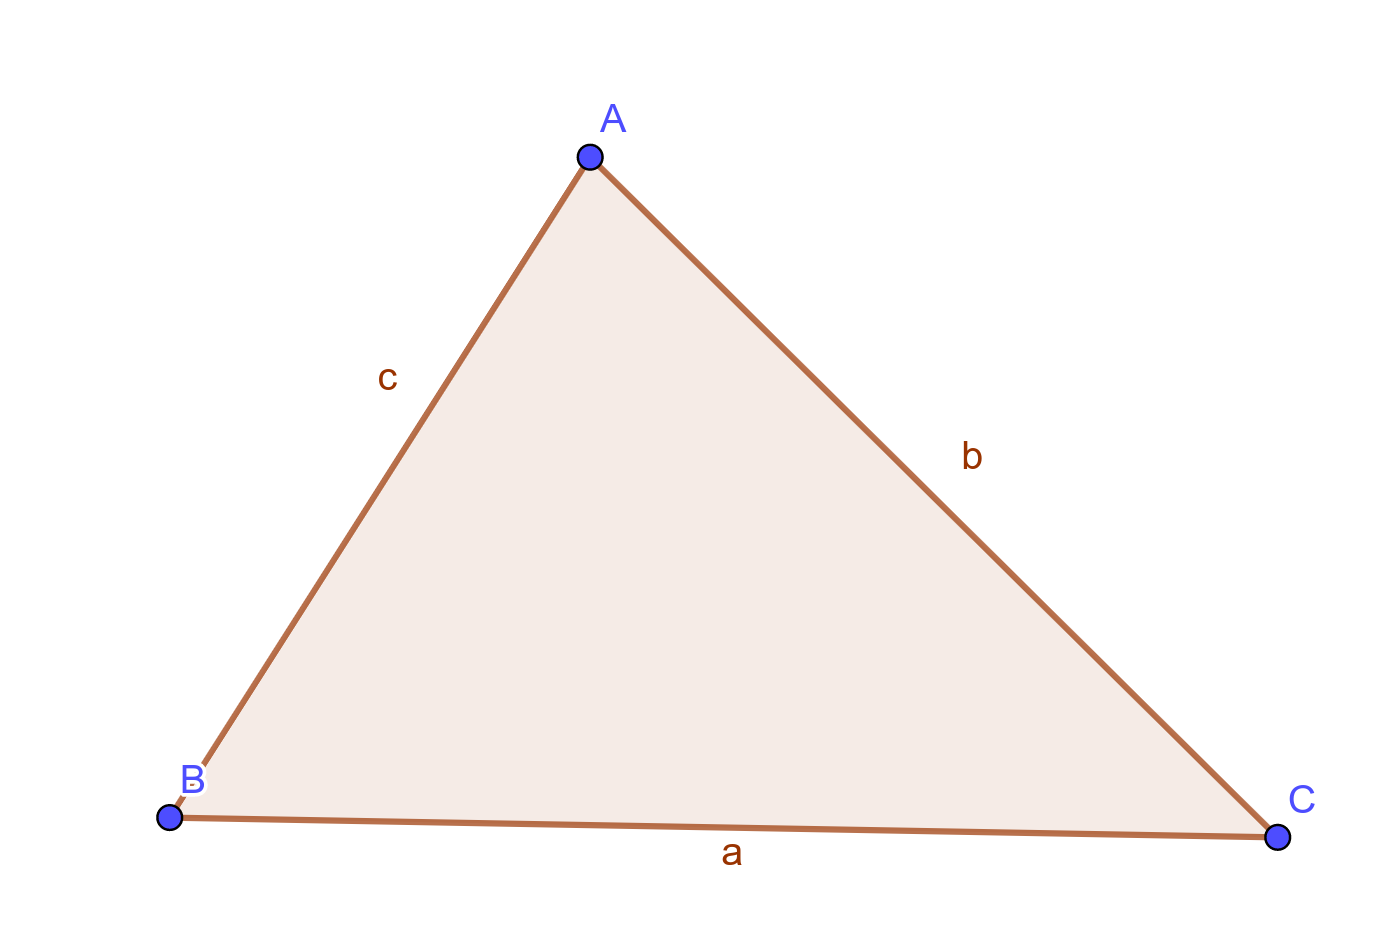
\includegraphics[width=8cm]{triangulo1.png}
    \caption{Triângulo \label{tria1}}
    
\end{figure}

\item $D$, $E$, e $F$ são os pés das alturas relativas aos lados $a$, $b$ e $c$ respectivamente.


\end{itemize} 


\section{Construindo os Pontos de Euler}

Considere o $\triangle ABC$ conforme a figura \ref{tria1} e nele traçamos as alturas relativas aos seus vértices, encontrando os pontos $D$, $E$, e $F$. Esses pontos são chamados de pés das alturas relativas.

\newpage

Considere agora a intersecção $O$ entre os três segmentos. Esta intersecção é o \textit{Ortocentro} do triângulo $ABC$

Considere os pontos médios $E_a$, $E_b$ e $E_c$ dos segmentos $AO$, $BO$ e $CO$ respectivamente neste triângulo conforme figura \ref{tria4}. Estes pontos médios são os pontos de Euler.

\begin{figure}[h]

    \center

    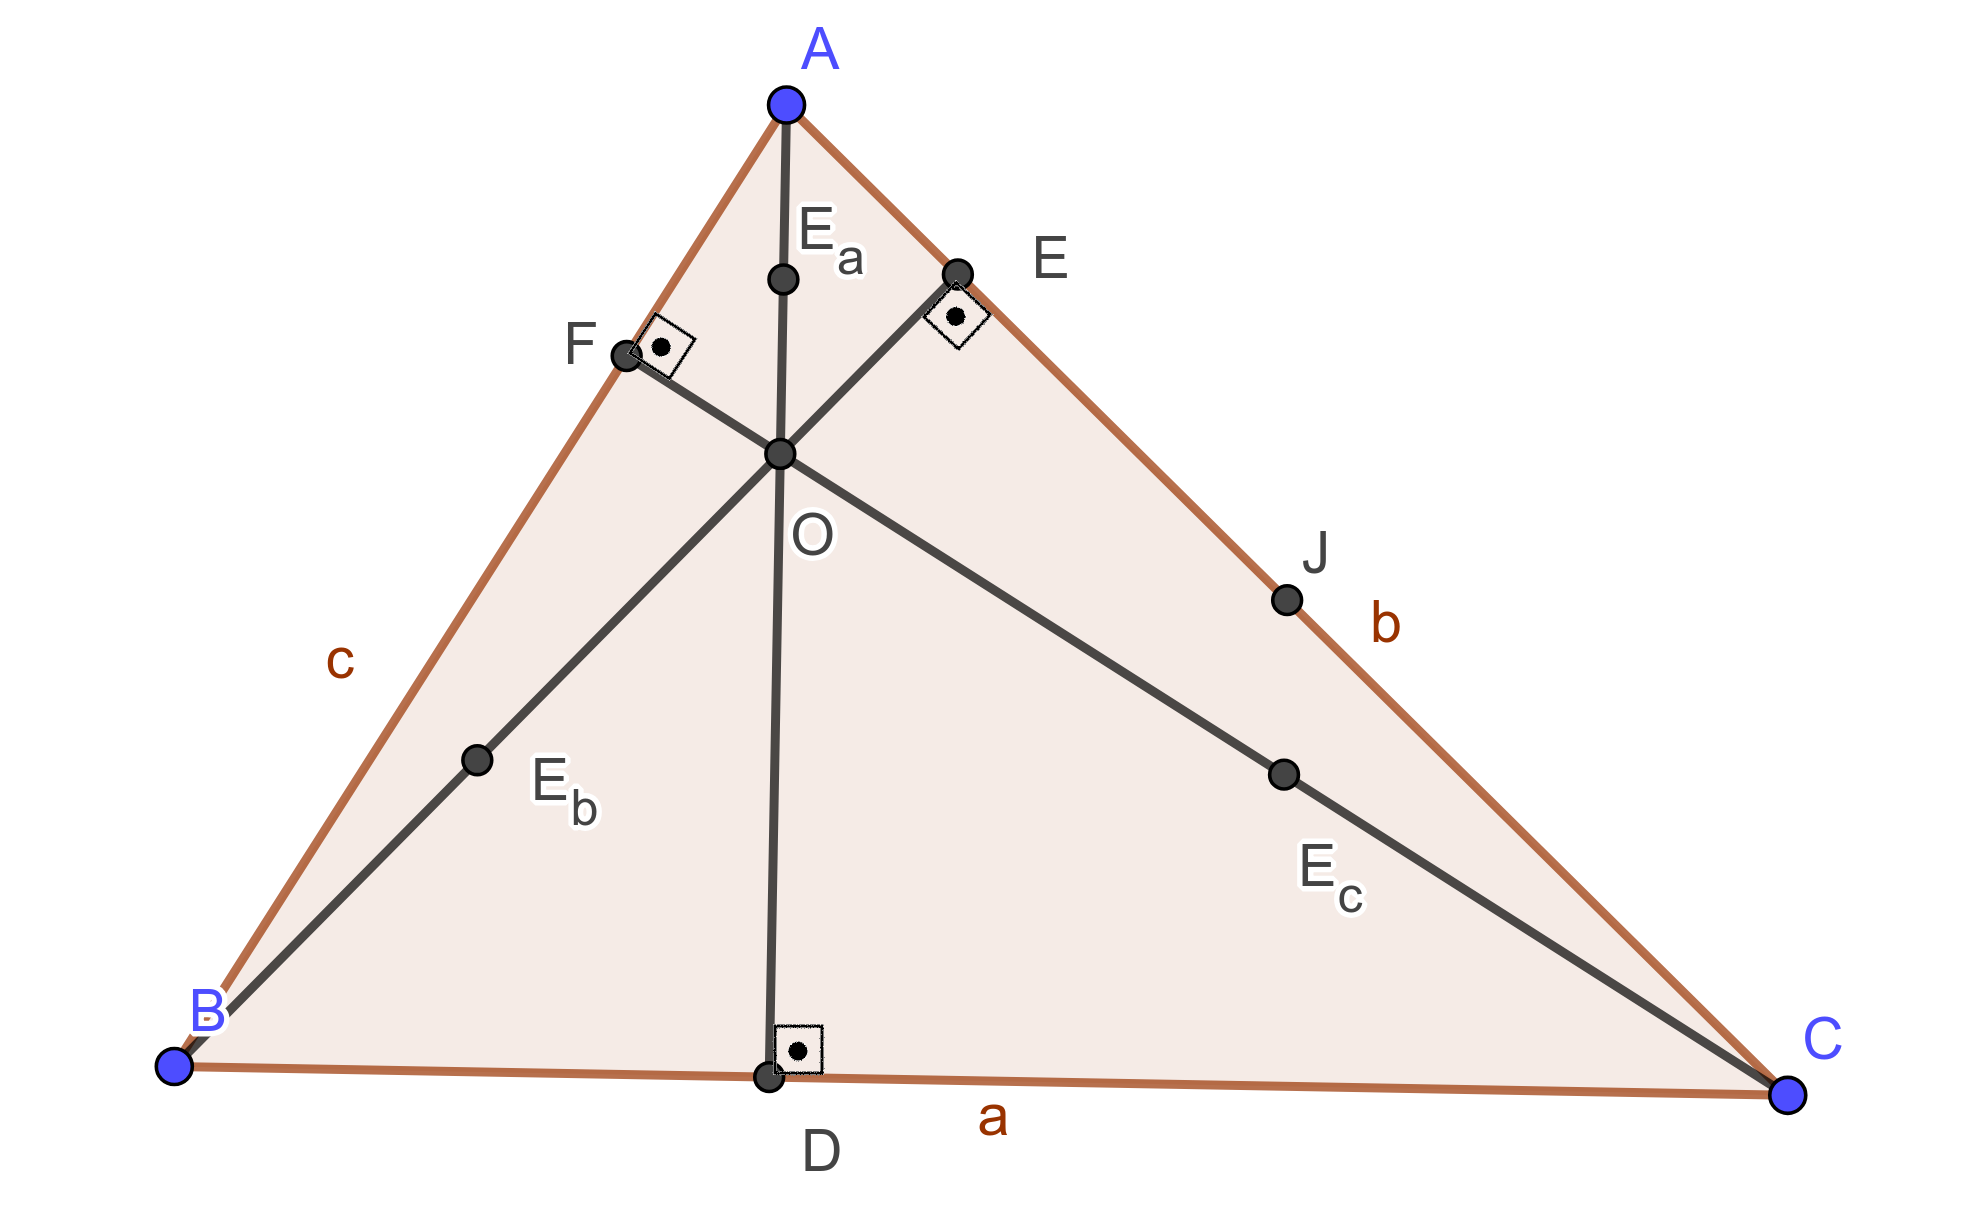
\includegraphics[width=9cm]{triangulo4.png}
    \caption{Alturas relativas e $\triangle DEF$ \label{tria4}}
    
\end{figure}

\chapter{A bissetriz e sua paralela}

Considere o triângulo $\triangle ABC$, com a bissetriz $AT_a$, altura $AH_a$, ponto médio $M_a$ relativo ao lado $BC$ e o ponto de Euler $E_a$, conforme figura \ref{triateo} . Faça um círculo de centro $E_a$ passando por $M_a$ de tal forma que intercepte a reta suporte de $AH_a$ no ponto $P$. Trace a linha $M_{a}P$.

\begin{teo}\label{teo1}
	Em qualquer triângulo $\triangle ABC$ com $H_a$ não coincidindo com $M_a$, o segmento $M_{a}P$ é paralelo a bissetriz $AT_a$
\end{teo}

\begin{figure}[h]
	
	\center
	
	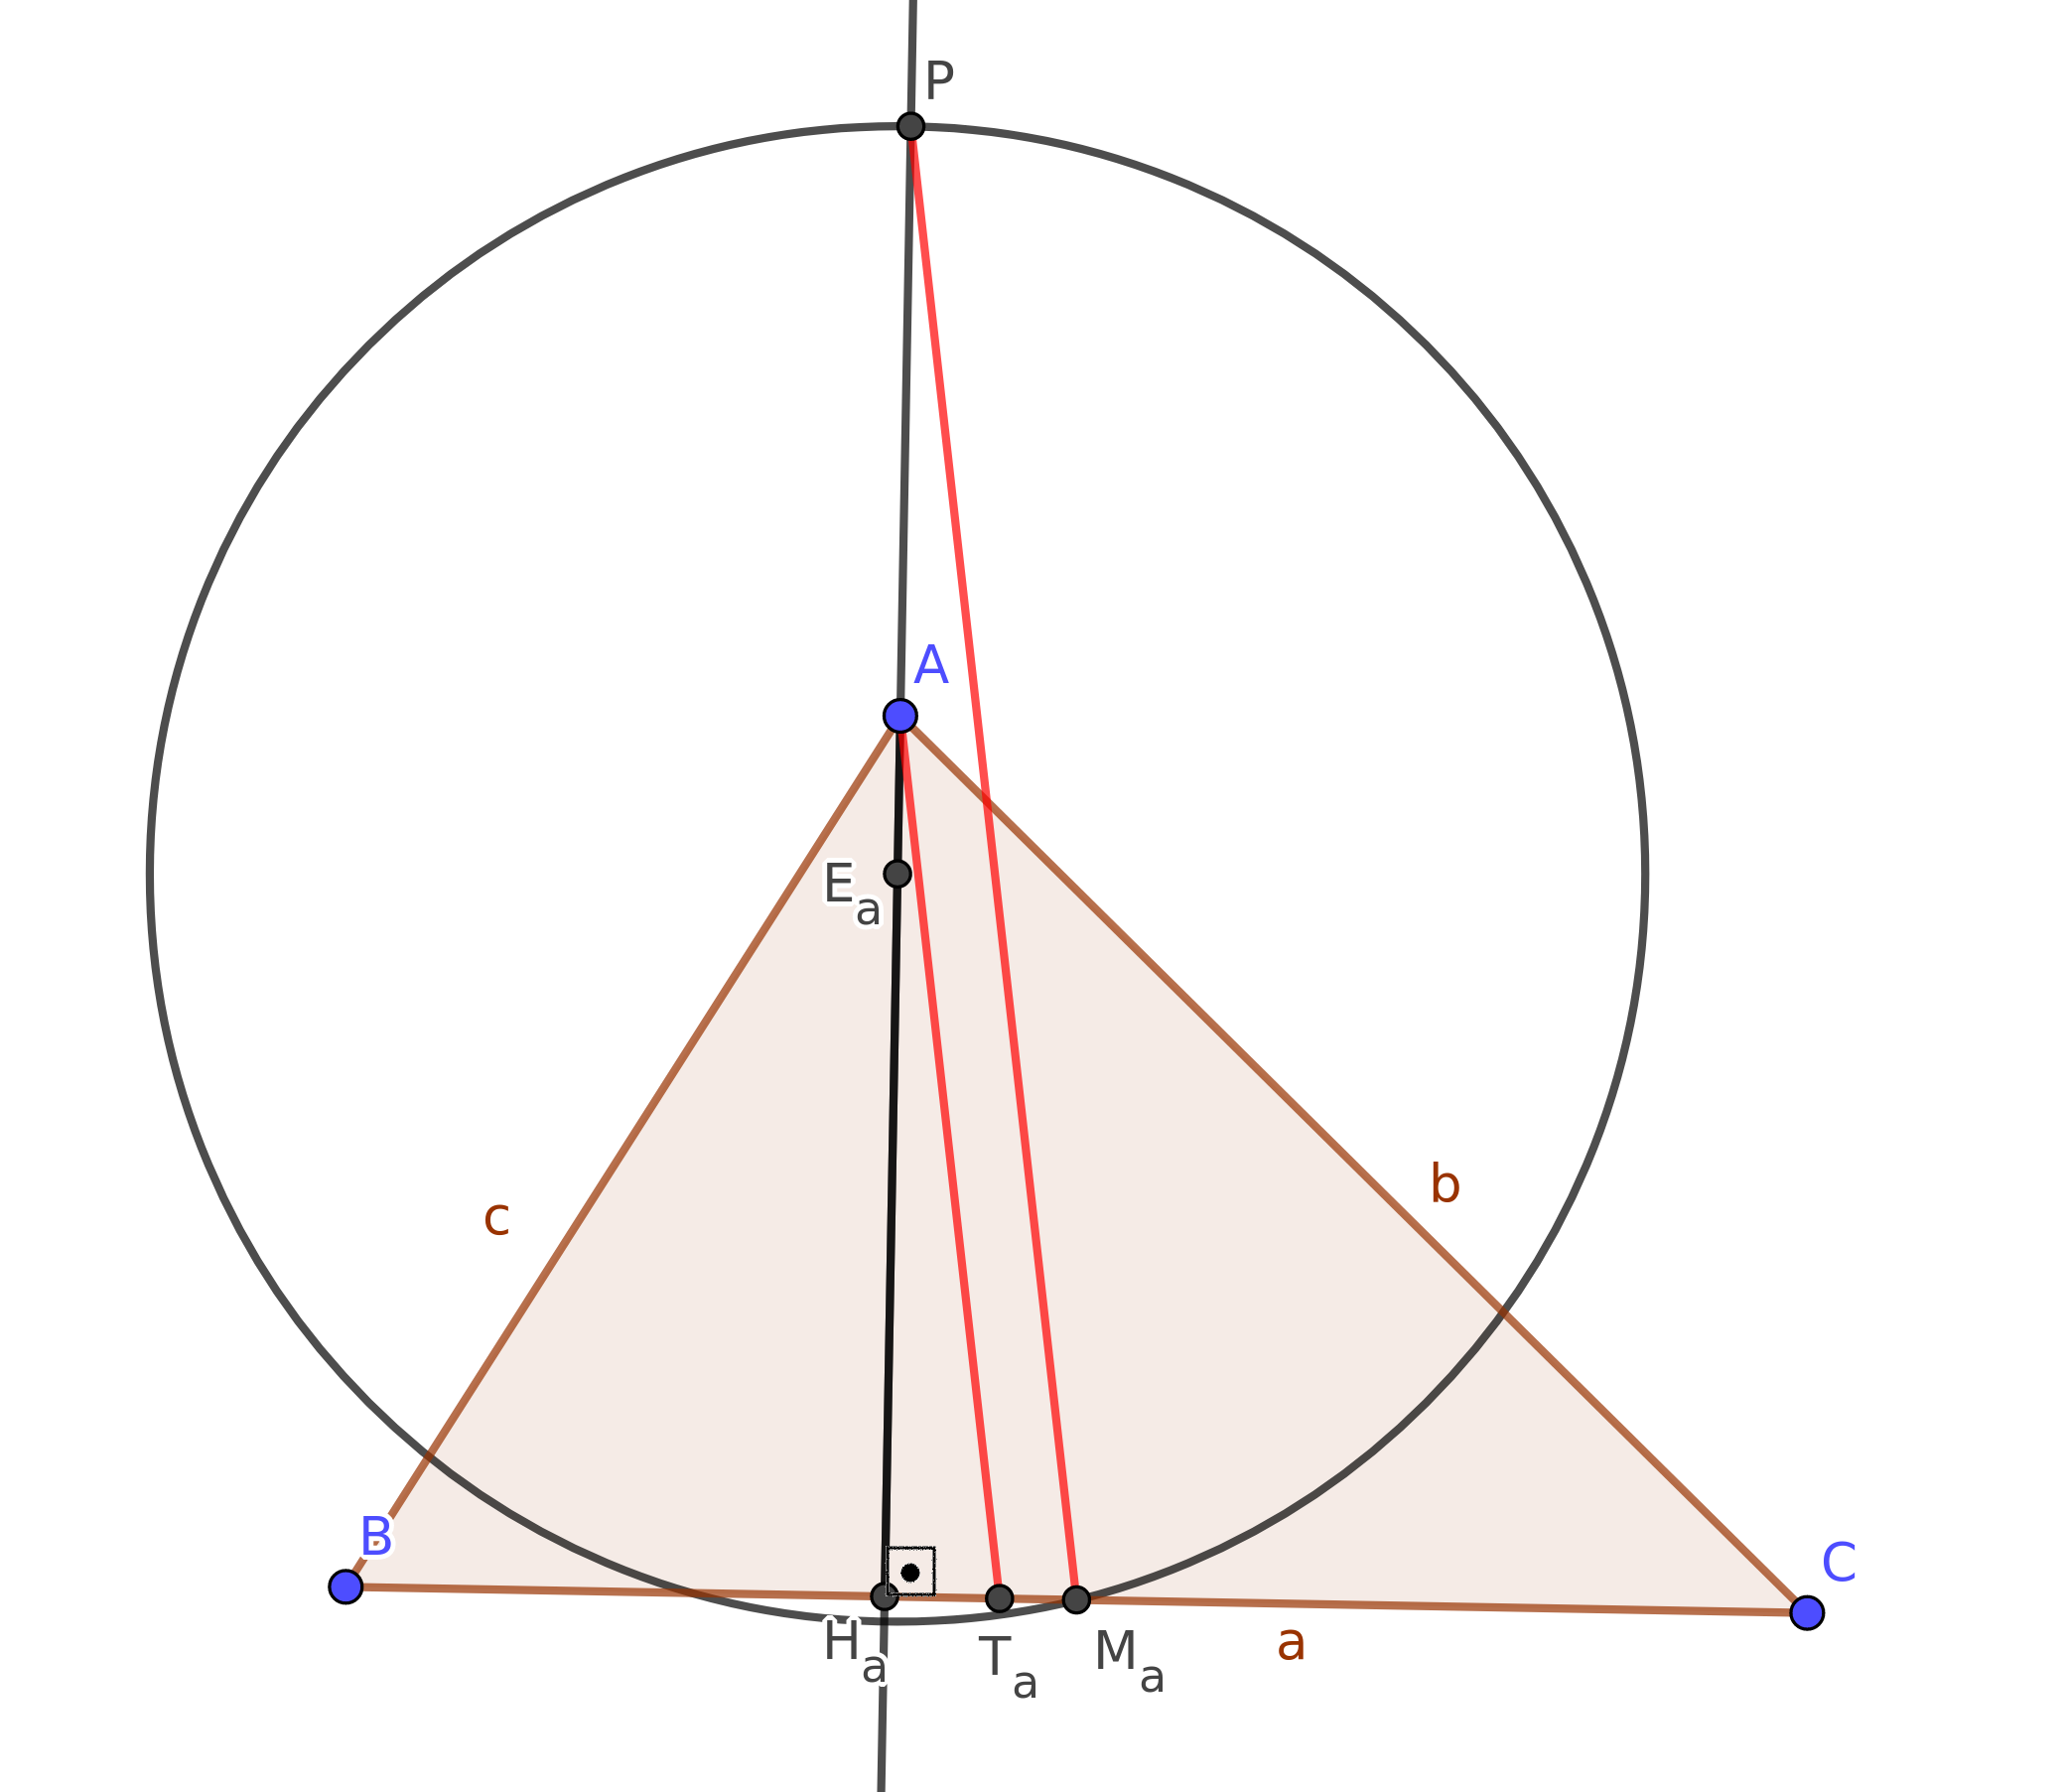
\includegraphics[width=8.5cm]{trianguloteo.png}
	\caption{Bissetriz e sua paralela \label{triateo}}
	
\end{figure}

\textit{Demonstração}

Seja $O$ o circuncentro do $\triangle ABC$. A mediatriz $M_{a}O$ e a bissetriz $AT_a$ intersecta o círculo circunscrito de centro $O$ em $S$, veja a figura \ref{trianbismed}:

\begin{figure}[h]
	
	\center
	
	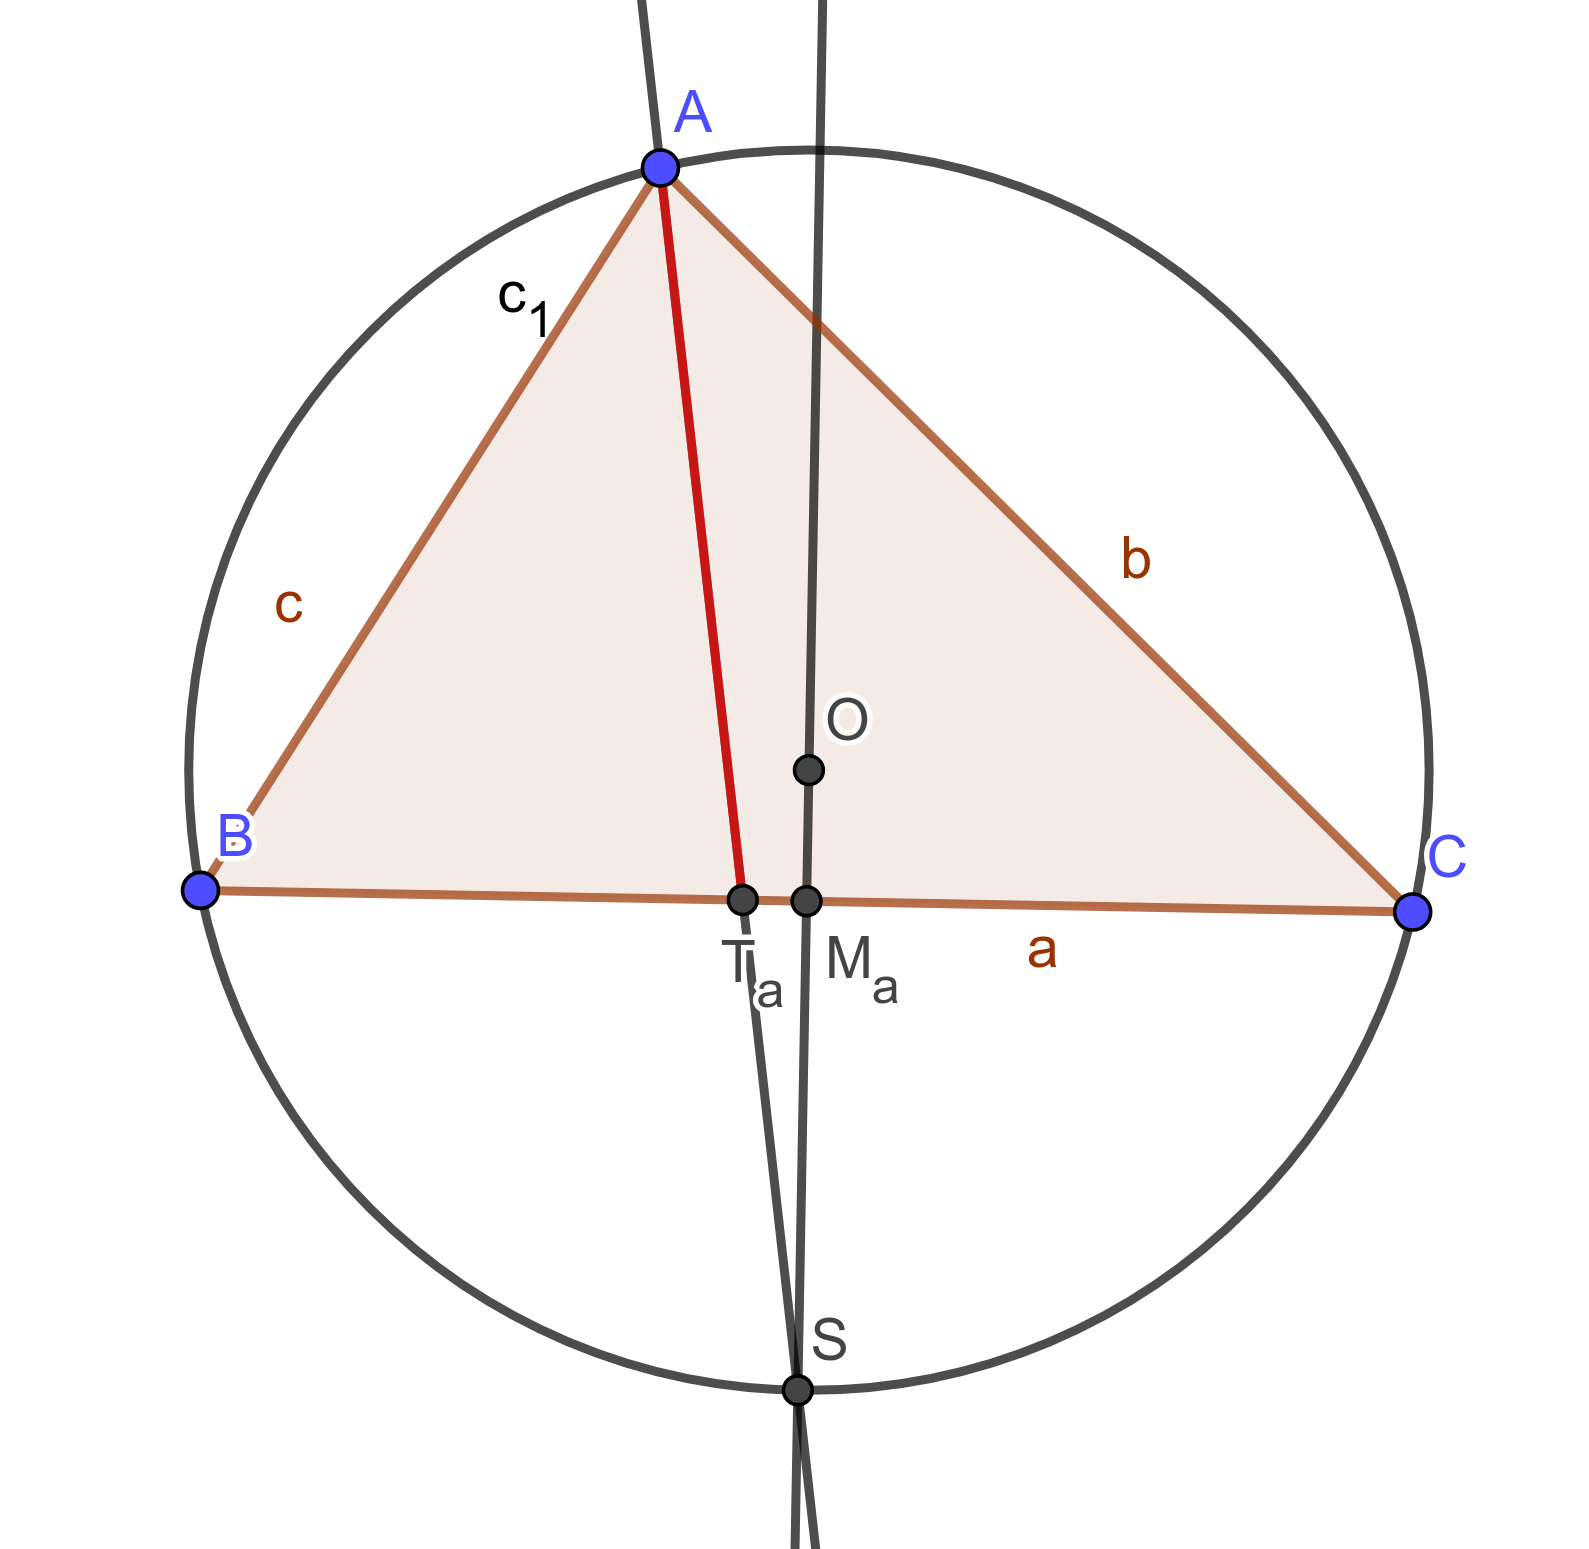
\includegraphics[width=5cm]{triangulocirc.png}
	\caption{Intersecção da bissetriz e da mediatriz\label{trianbismed}}
	
\end{figure}

O ângulo $\hat{BAC}$ tem como arco de visada o arco $BC$. Como $AT_a$ é a bissetriz de $\hat{BAC}$ irá intersectar o círculo de centro $O$ no ponto médio do arco de visada $AB$. A mediatriz $OM_a$ é o lugar geométrico em que todos os pontos estão equidistantes dos pontos $B$ e $C$, logo o ponto em que esta intersecta o círculo de centro $O$ também é equidistante desses pontos, assim também é metade do arco $BC$, logo a mediatriz $OM_a$ e a bissetriz $AT_a$ se intersectam no ponto $S$ contido no círculo de centro $O$.

Agora seja $R$ o ponto médio do segmento $E_{a}O$ e faça a reflexão de toda a figura \ref{trianbismed} com centro em $R$. Seja o  $\triangle A'B'C'$ a reflexão do $\triangle ABC$, conforme a figura \ref{trianref}.

\begin{figure}[h]
	
	\center
	
	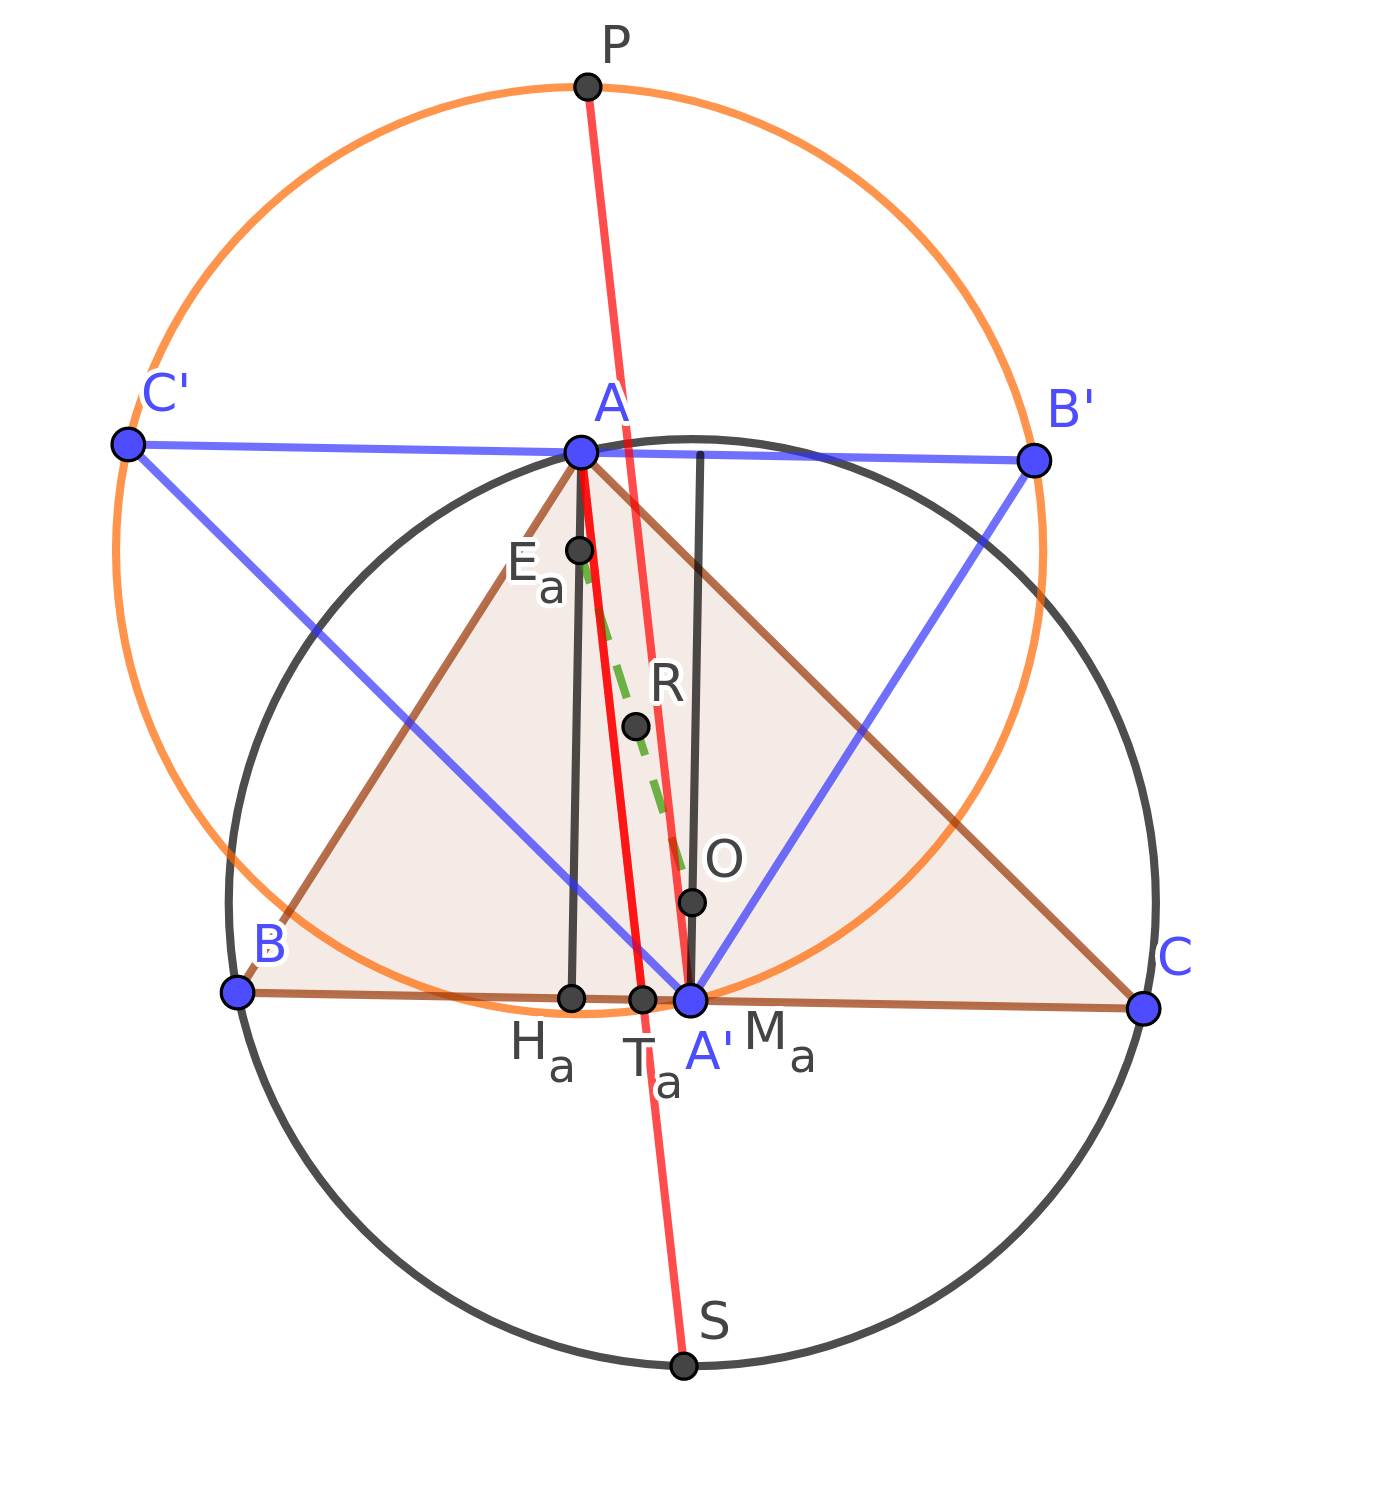
\includegraphics[width=8.5cm]{trianreflexao.png}
	\caption{Reflexão do $\triangle ABC$ \label{trianref}}
	
\end{figure}

Note que, como $R$ é ponto médio de $E_{a}O$, a reflexão de $E_a$ é o próprio ponto $O$ e a reflexão do segmento que passa por $E_a$ saindo do vértice $A$ é o segmento que passa por $O$ saindo de $M_a$, logo o vértice $A'$ coincide com o ponto $M_a$. Desta forma o círculo circunscrito ao $\triangle A'B'C'$ passa também por $M_a$ e tem raio $E_{a}M_{a}$, desta forma, o círculo de centro $E_a$ passando por $M_a$ é a reflexão do círculo circunscrito ao $\triangle ABC$ de centro $O$. Da mesma forma, os segmentos $AE_a$ e $M_{a}O$ são iguais e paralelos, $A$ é a reflexão de $M_a$ logo é o ponto médio de $B'C'$. Portanto $AH_a$ é a mediatriz de $B'C'$. Por fim, $AH_a$ intersecta o círculo de centro $E_a$ e raio $M_a$ em $P$, portanto $M_aP$ é a bissetriz do ângulo $\hat{B'A'C'}$ e paralelo a $AT_a$.

\textit{Observação}: Quando $H_a$ e $M_a$ coincidirem, o triângulo é isósceles em $A$ ou equilátero, então os segmentos $M_{a}P$ e $AT_a$ serão coincidentes.

\chapter{Resolvendo problemas}

Wernick\cite{Wernick} apresentou 139 problemas de construção de triângulos com régua e compasso dada a localização de três pontos associados ao triângulo escolhidos de uma lista de dezesseis pontos. Veja Meyers\cite{Meyers} para atualizações sobre o status dos problemas desta lista. Connelly \cite{con} estendeu este trabalho adicionando mais quatro pontos à lista e 140 problemas adicionais, muitos dos quais foram designados como não resolvidos. Agora aplicamos o Teorema \ref{teo1} para resolver quatros desses problemas anteriormente não resolvidos. Os números dos problemas são dados por Connelly.

\section{Problema 99}

Dados os pontos $E_a$, $M_a$ e $T_a$ construir o triangulo $\triangle ABC$.

\textit{Solução}: Trace a linha $M_{a}T{a}$ contida no lado BC e então a altura $E_{a}H_{a}$ relativa a esse lado. O círculo com centro em $E_{a}$ passando por $M_{a}$ intersecta a altura em $P$. Desenhe $M_{a}P$. Pelo teorema \ref{teo1}, o segmento passando em $T_{a}$ paralela por $M{a}P$ intersecta a altura em $A$. Faça a reflexão de $A$ através de $E_{a}$. $E_{a}$ é o ponto médio entre o ortocentro e o vértice A, logo esta reflexão será o ortocentro do $\triangle ABC$ (veja figura \ref{trianexer}). O ponto médio de $E_{a}M_{a}$ será o ponto $N$. Refletindo $H$ através do ponto $N$ obtém-se o ponto $O$, que será o circuncentro do $\triangle ABC$. Assim, desenhando o círculo com centro em $O$ passando por $A$ intersectará a reta suporte de $M_{a}T_{a}$ em $B$ e $C$. 

\begin{figure}[h]
	
	\center
	
	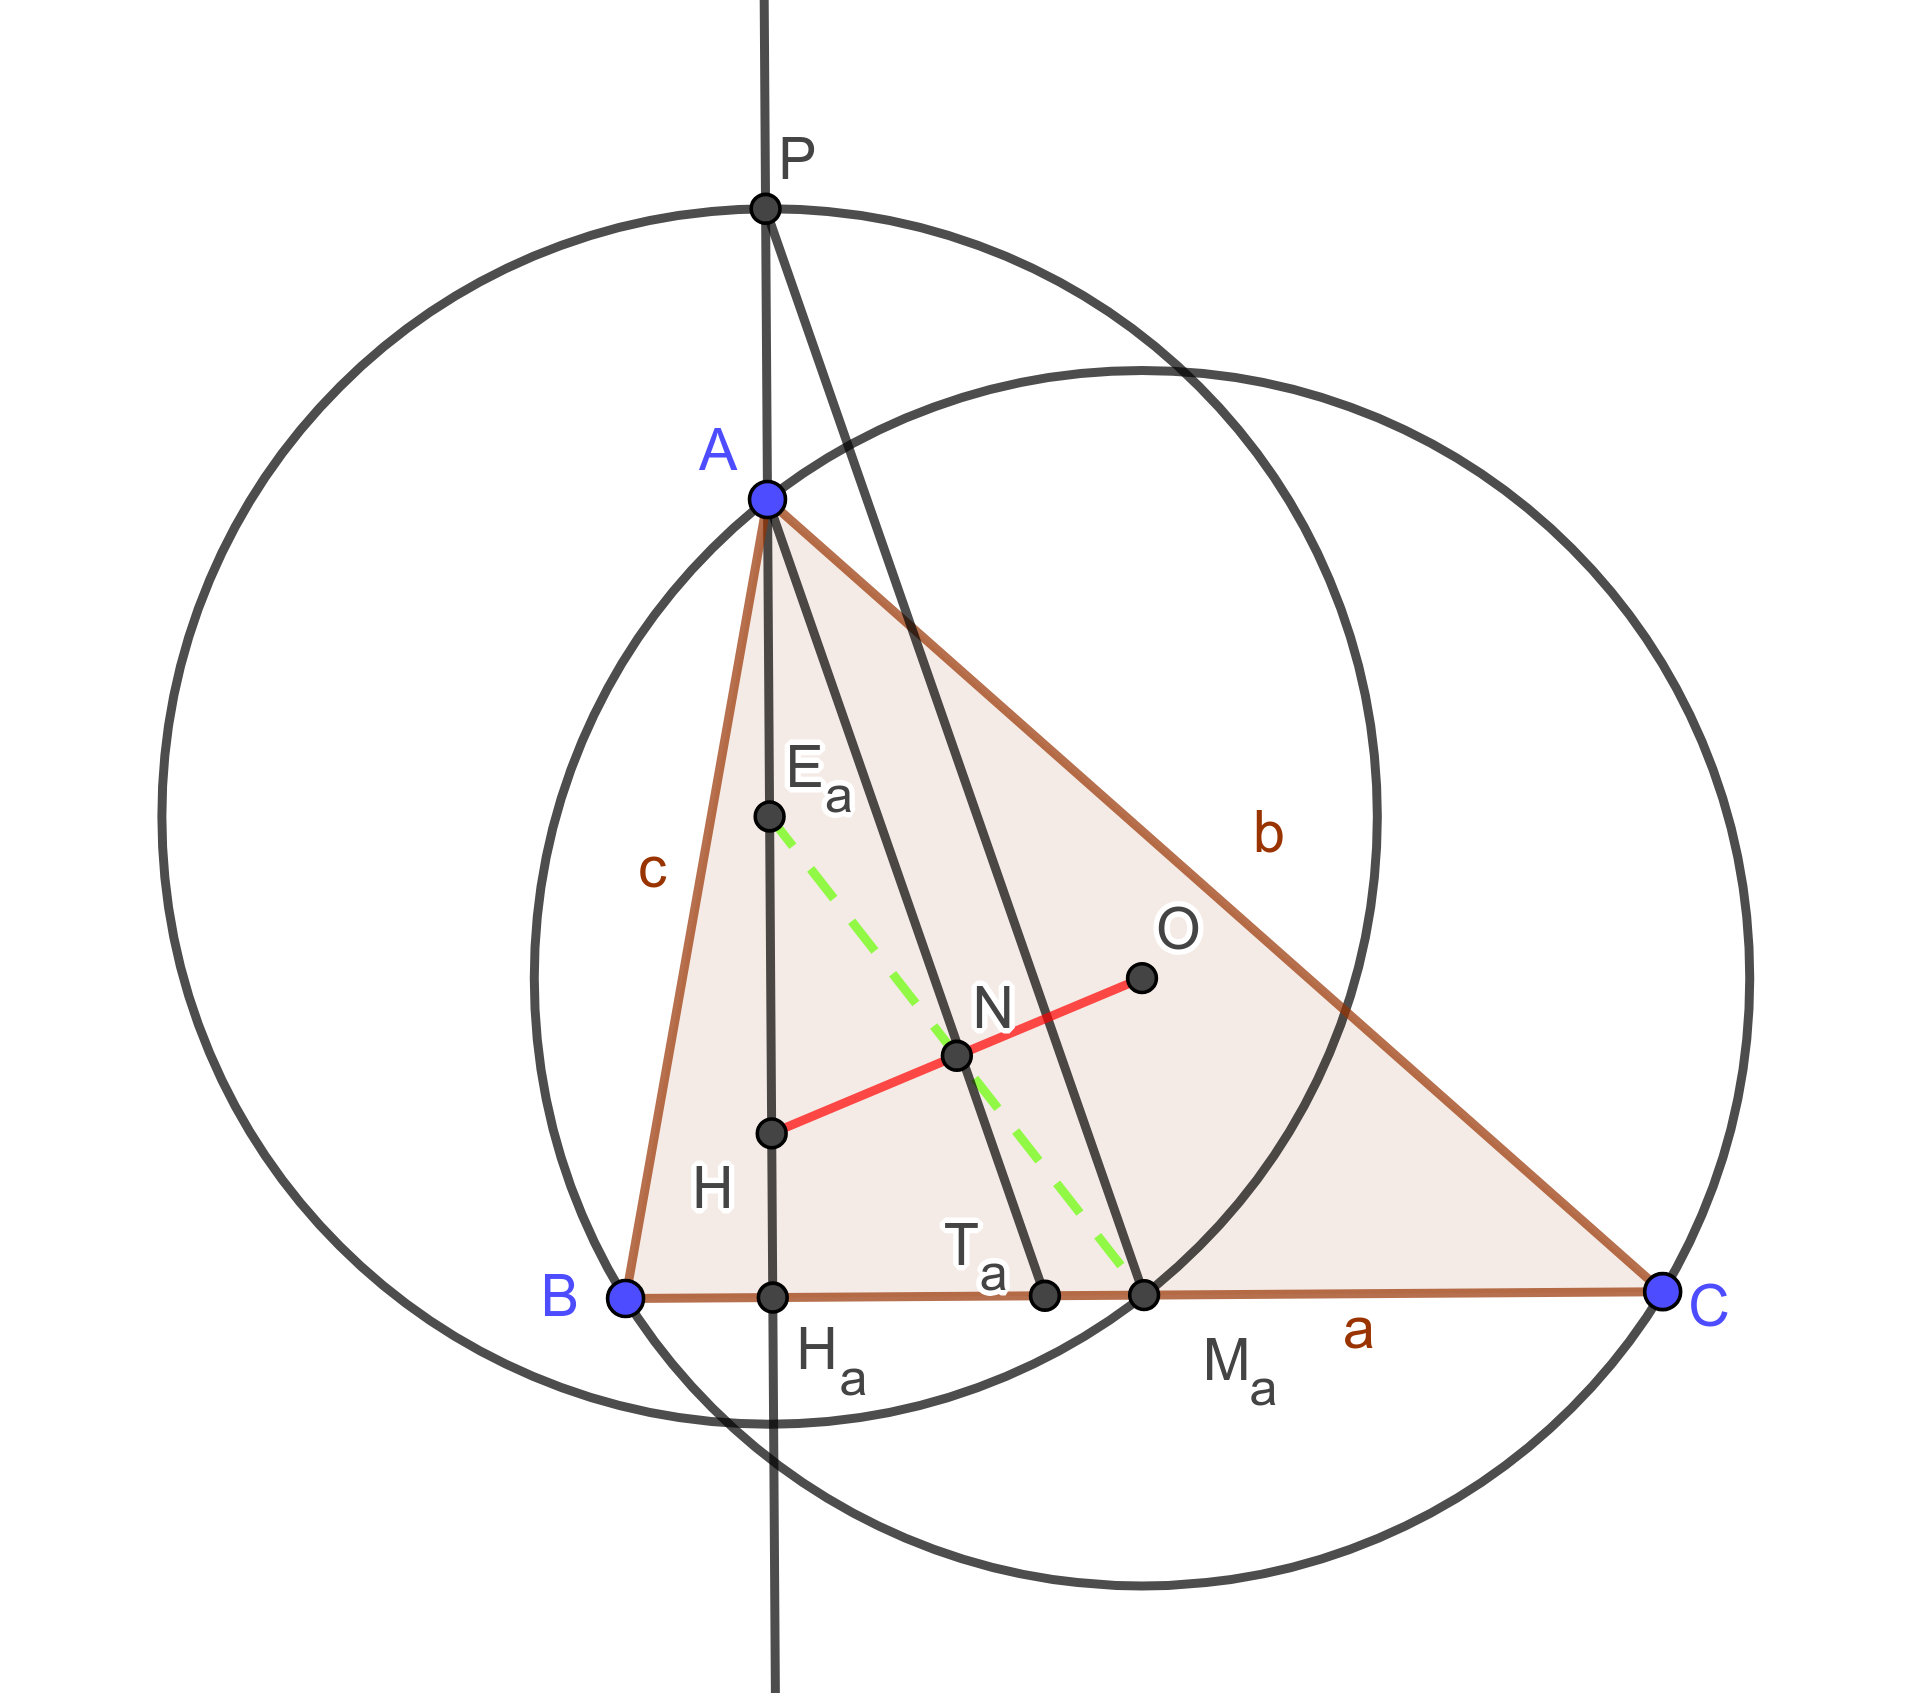
\includegraphics[width=9cm]{triangexer.png}
	\caption{Reflexão do $\triangle ABC$ \label{trianexer}}
	
\end{figure}


\textit{Número de Soluções}: Dependendo da posição relativa dos três pontos, o exercício tem duas soluções, nenhuma solução ou um número infinito de soluções. Começamos localizando $E_{a}$ e $M_{a}$. Então o segmento $E_{a}M_{a}$ é um diâmetro do círculo de nove pontos com centro em $N$ (conforme Mesquita\cite{mesquita2013}). Como, para qualquer triângulo, o ângulo $\hat{E_{a}T_{a}M_{a}}$ deve ser maior que $90^\circ$, $T_a$ deve estar dentro do círculo, ou coincide com $M_a$, para ter uma solução válida. Para o caso com $T_a$ dentro do círculo, temos duas soluções, já que o círculo de centro $E_{a}$ passando por $M_a$ cruza a altitude duas vezes e cada intersecção leva a uma solução distinta. Se os três pontos são colineares, os dois triângulos são reflexos congruentes entre si através da reta. Se $T_a$ é fora ou no círculo de nove pontos, exceto em $M_a$, não há solução. Se $T_a$ coincide com $M_a$, há um número infinito de soluções. Neste caso, o vértice A pode ser escolhido em qualquer lugar no segmento aberto $M_{a}M_{a}'$ (onde $M_{a}'$ é o reflexo de $M_{a}$ através de $E_a$), e há um triângulo isósceles resultante.

\section{Problema 108}

Dado os pontos $E_a$, $N$ e $T_a$, construir o triângulo $ABC$.

\textit{Solução}: Como $N$ é o ponto médio entre $E_a$ e $M_a$, faça a reflexão de $E_a$ por $N$, assim temos o ponto $M_a$ e assim o exercício será idêntico ao anterior.

\section{Problema 137}

Dado os pontos $M_a$, $N$ e $T_a$ construir o triângulo $ABC$.

\textit{Solução}: Da mesma forma que o problema anterior, faça a reflexão de $M_a$ por $N$ e assim temos o ponto $E_a$ e, novamente, o problema se reduz ao problema 99.

\section{Problema 130}

Dado os pontos $H_a$, $N$ e $T_a$ construir o triângulo $ABC$.

\textit{Solução}: O círculo de nove pontos, com centro em $N$ passando por $H_a$, intersecta a linha $H_{a}T_{a}$ em $M_a$ (conforme Mesquita\cite{mesquita2013}), assim temos os mesmos pontos do problema 137.

\bibliography{bibliografia}

\end{document}
